\documentclass[forprint]{WHUBachelor}

\begin{document}
\CollegeName{XX大学}
\ECollegeName{XX University}
\ConfidentialLevel{}                                      % 密级
\StudentNumber{15XXXXXXXX} % 学号
\title{基于XXXX的XXXX}
\Etitle{A XXXX Based On XXXX} % 英文题目
\author{Arsennnic}                            % 作者名字
\Eauthor{Arsennnic}            %作者英文名
\Csupervisor{XXX\quad 教授}        %指导教师中文名、职称
\Esupervisor{Prof.~XXX}     %指导教师英文名、职称
\Cmajor{动力机械及工程}                  % 专业中文名
\Emajor{Power Machinery and Engineering}% 专业英文名
\Cschoolname{能源与动力工程学院}          % 学院名
\Eschoolname{School of Energy and Power Engineering} %学院英文名
\date{二〇一八年五月}                    % 日期, 要注意和英文日期一致!!
\Edate{May, 2018}                       % 英文封面日期


\pdfbookmark[0]{封面}{title}			%封面页加到 pdf 书签
\maketitle
\frontmatter
\pagenumbering{Roman}					%正文之前的页码用大写罗马字母编号.
% !Mode:: "TeX:UTF-8"

%%% 此部分需要自行填写: (1) 中文摘要及关键词 (2) 英文摘要及关键词
%%%%%%%%%%%%%%%%%%%%%%%%%%%%%
%%% -------------  英文封面 (无需改动)-------------   %%%
%%%%%%%%%%%%%%%%%%%%%%%%%%%%%
\thispagestyle{empty}
\renewcommand{\baselinestretch}{1.5}  %下文的行距
\vspace*{0.5cm}
\begin{center}
{\Large \bf BACHELOR'S DEGREE THESIS \\[1ex] OF \the\ECollegeName }
\end{center}
\vspace{2.5cm}
\begin{center}{\zihao{2} \the\Etitle \par}\end{center}

\vfill

\begin{center}
\zihao{4}
\begin{tabular}{ r l }
 School (Department): & {\sc \the\Eschoolname}\\
  Major:          &   {\sc\the\Emajor}  \\
 Candidate:      &  {\sc \the\Eauthor}  Name    \\
 Supervisor:     &  {\sc \the\Esupervisor}
\end{tabular}

\vspace*{2cm}
\begin{center}

\includegraphics[height=4cm]{logo.png}
\end{center}


\zihao{-2}
%\the\Schoolname\\
{\sc \the\ECollegeName}

\vspace*{1.0cm}

\the\Edate

\end{center}
%%% 郑重声明部分无需改动

%%%---- 郑重声明 (无需改动)------------------------------------%
\newpage
\vspace*{20pt}
\begin{center}{\ziju{0.8}\textbf{\songti\zihao{2} 郑重声明}}\end{center}
\par\vspace*{30pt}
\renewcommand{\baselinestretch}{2}

{\zihao{4}%

本人呈交的学位论文, 是在导师的指导下, 独立进行研究工作所取得的成果,
所有数据、图片资料真实可靠. 尽我所知, 除文中已经注明引用的内容外,
本学位论文的研究成果不包含他人享有著作权的内容.
对本论文所涉及的研究工作做出贡献的其他个人和集体,
均已在文中以明确的方式标明. 本学位论文的知识产权归属于培养单位.\\[2cm]

\hspace*{1cm}本人签名: $\underline{\hspace{3.5cm}}$
\hspace{2cm}日期: $\underline{\hspace{3.5cm}}$\hfill\par}
%------------------------------------------------------------------------------
\baselineskip=23pt  % 正文行距为 23 磅
%------------------------------------------------------------------------------





%%======中文摘要===========================%
\begin{cnabstract}
本文主要介绍和讨论了\the\CollegeName 本科毕业论文的~\LaTeX~模板.
指明了编译方法, 强调了公式排版的一些细节问题, 也指出了一些常见的排版错误.



\end{cnabstract}
\par
\vspace*{2em}


%%%%--  关键词 -----------------------------------------%%%%%%%%
%%%%-- 注意: 每个关键词之间用“;”分开,最后一个关键词不打标点符号
\cnkeywords{毕业论文; \LaTeX{}; 模板;  }


%%====英文摘要==========================%


\begin{enabstract}
This thesis is a study on the theory of \dots.

\end{enabstract}
\par
\vspace*{2em}

%%%%%-- Key words --------------------------------------%%%%%%%
%%%%-- 注意: 每个关键词之间用“;”分开,最后一个关键词不打标点符号
 \enkeywords{\LaTeX{};  }

\pdfbookmark[0]{目录}{toc}
\tableofcontents
\mainmatter


\chapter{模板使用教程}
 
 \section{具体使用步骤}

 \begin{description}

  \item[Step 1]  进入 includefile 文件夹,打开 frontmatter.tex, backmatter.tex 这两个文档,分别填写中文摘要、英文摘要、致谢;

  \item[Step 2]  进入 figure 文件夹,把学校logo换掉;

  \item[Step 3]  打开主文档 Bachelor--template.tex, 填写题目、作者等等信息,书写正文。


\end{description}


\section{编译的方法}\label{sec-compile}

默认使用 XeLaTeX 编译, 直接生成~pdf 文件.

若另存为新文档, 请确保文档保存类型为 \verb|:UTF-8|. 当然目前很多编辑器默认文字编码为 UTF-8.
WinEdt 9.0 之后的版本都是默认保存为 UTF-8 的.


\vfill
本文档由武汉大学@黄正华(\url{http://aff.whu.edu.cn/huangzh/})初次编写,由@Arsennnic(\url{https://github.com/Arsennnic/latex-template-degree-thesis})二次修改。问题反馈及建议请联系:arsennnic@gmail.com


\chapter{\LaTeX 基本命令}
\section{字体调节}

\begin{tabular}{ll}
	\verb|\songti|   & {\songti 宋体}   \\
	\verb|\heiti|    & {\heiti 黑体}    \\
	\verb|\fangsong| & {\fangsong 仿宋} \\
	\verb|\kaishu|   & {\kaishu 楷书}
\end{tabular}


\section{字号调节}

\begin{tabular}{ll}
	\verb|\zihao{0}| &\zihao{0}  初号字 English \\
	\verb|\zihao{-0}|&\zihao{-0} 小初号 English \\
	\verb|\zihao{1} |&\zihao{1}  一号字 English \\
	\verb|\zihao{-1}|&\zihao{-1} 小一号 English \\
	\verb|\zihao{2} |&\zihao{2}  二号字 English \\
	\verb|\zihao{-2}|&\zihao{-2} 小二号 English \\
	\verb|\zihao{3} |&\zihao{3}  三号字 English \\
	\verb|\zihao{-3}|&\zihao{-3} 小三号 English \\
	\verb|\zihao{4} |&\zihao{4}  四号字 English \\
	\verb|\zihao{-4}|&\zihao{-4} 小四号 English \\
\end{tabular}


\section{参考文献的引用}

参考文献的引用, 用命令~\verb|\cite{ }|. 大括号内要填入的字串, 是自命名的文献条目名. 此外,自定义了~\verb|\upcite| 命令, 使文献引用呈现为\CJKunderdot{上标形式}. 比如, 通常我们会说:

{\kaishu
	关于此问题, 请参见文献 \cite{r2}. 作者某某还提到了某某概念\upcite{r1}.}

\noindent
其\LaTeX 源代码为:

{\kaishu
	关于此问题, 请参见文献~\verb|\cite{r2}|. 作者某某还提到了某某概念~\verb|\upcite{r1}|.
}


\section{图形与表格}

用形如~\verb|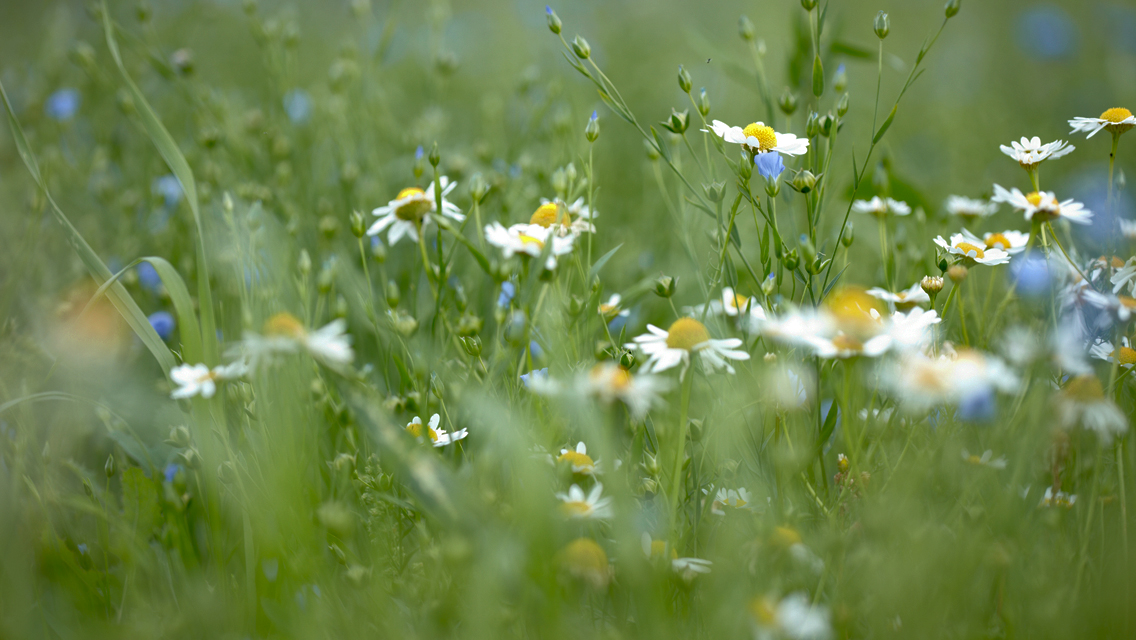
\includegraphics[width=12cm]{Daisy.jpg}| 的命令可以纳入图片.

如图~\ref{fig:1} 是一个纳入~jpg 图片的例子.

\begin{figure}[ht]
	\centering
	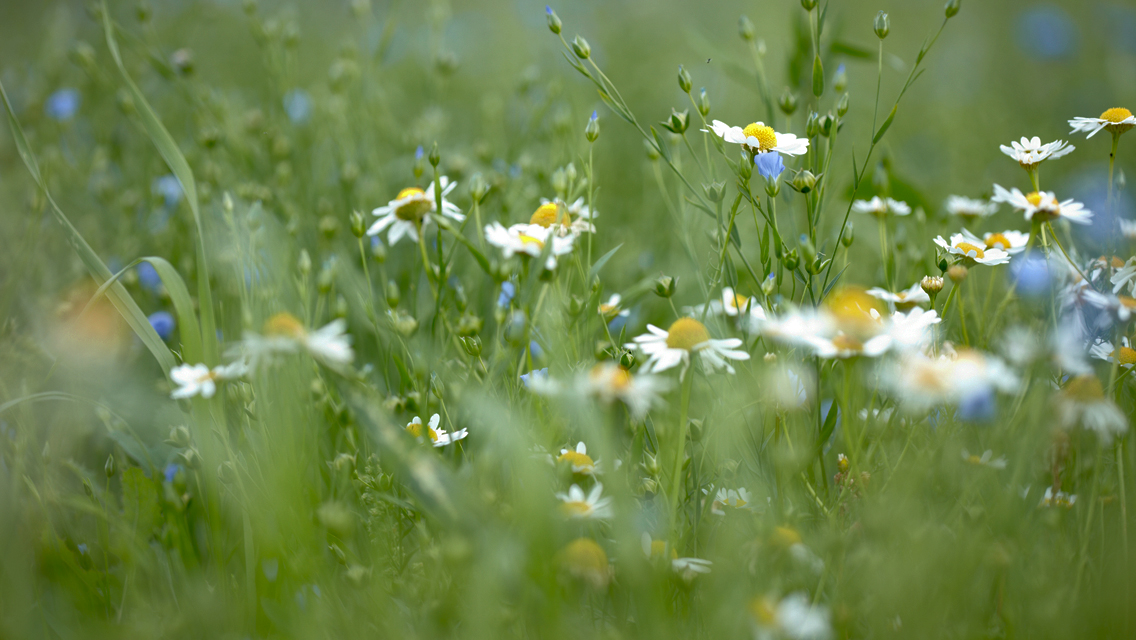
\includegraphics[width=0.6\textwidth]{Daisy.jpg}
	\caption{一个彩色 jpg 图片的例子}
	\label{fig:1}
\end{figure}

表格建议使用“三线表”, 如表 \ref{tab:1}.

\begin{table}[ht]
	\centering
	\caption{一般三线表}
	\label{tab:1}
	\begin{tabular}{c c c c c c c c c c c}
		\hline
		123 & 4  & 5  & 123 & 4 & 5123 & 4 & 5 & 123 & 4 & 5\\
		\hline
		67 & 890 & 13 & 123 & 4 & 5123 & 4 & 5 & 123 & 4 & 5\\
		67 & 890 & 13 & 123 & 4 & 5123 & 4 & 5 & 123 & 4 & 5\\
		67 & 890 & 13 & 123 & 4 & 5123 & 4 & 5 & 123 & 4 & 5\\
		\hline
	\end{tabular}
\end{table}



\cleardoublepage\phantomsection
\addcontentsline{toc}{chapter}{参考文献}
\begin{thebibliography}{00}

  \bibitem{r1} 作者. 文章题目 [J].  期刊名, 出版年份,卷号(期数): 起止页码.

  \bibitem{r2} 作者. 书名 [M]. 版次. 出版地:出版单位,出版年份:起止页码.


\end{thebibliography}

% !Mode:: "TeX:UTF-8"
%%%%%%%%%%%%%%%%%%%%%%%%%%%%-------致谢--------%%%%%%%%%%%%%%%%%%%%%%%%%%%%%%%%

\acknowledgement
\addcontentsline{toc}{chapter}{致谢}


感谢你, 感谢他和她, 感谢大家.











 

\appendix

\chapter{第一个附录}


\chapter{第二个附录}

\cleardoublepage
\end{document}



